\documentclass{article}
\usepackage{verbatim}
\usepackage{fullpage}
\usepackage{amsmath}
\usepackage{graphicx}
\usepackage{listings}
\usepackage{placeins} % for \FloatBarrier
%% package for contiued float
\usepackage{caption}
\usepackage[english,greek, main=greek]{babel}
\usepackage[utf8]{inputenc}
\useshorthands{;}
\defineshorthand{;}{?}

\usepackage[explicit]{titlesec} % number after section name
\titleformat{\section}
  {\normalfont\large\bfseries}
  {}
  {0em}
  {#1\ \thesection}
%% number after subsection name
\titleformat{\subsection}
  {\normalfont\large\bfseries}
  {}
  {0em}
  {#1\ \thesubsection}
%% number after subsection name
\titleformat{\section}
  {\normalfont\Large\bfseries}
  {}
  {0em}
  {\ifnum\value{section}=0\relax #1\else #1\ \thesection\fi}
\newcommand{\eng}[1]{\foreignlanguage{english}{#1}} % shortcut for inserting english into greek text


\title{
    \includegraphics[width=\textwidth]{~/Pictures/emp.png} \\
    \vskip 5cm
    Νευροασαφής Έλεγχος και Εφαρμογές\\
    \large Άσκηση 4η
    \vskip 5cm
}

\author{Αναστάσιος Στέφανος Αναγνώστου\\
        03119051}

\begin{document}

\maketitle
\newpage
\tableofcontents
\newpage

\section{Θέμα}

\subsection{Ερώτημα}

Δεν απαντήθηκε.

%% \selectlanguage{english}
%% \begin{lstlisting}[language=Python]
%% import numpy as np
%% 
%% def markov_chain(a, b, c):
%%     chain = np.array([
%%         [0, 1 - a - b, a, b, 0],
%%         [0, 0, 1, 0, 0],
%%         [0, 0, 0, 1 - c, c],
%%         [1, 0, 0, 0, 0],
%%         [0, 0, 0.5, 0, 0.5]
%%     ])
%%     for transition_probabilities in chain:
%%         assert sum(transition_probabilities) == 1
%%     return chain
%% 
%% if __name__ == '__main__':
%%     # c can be anything from 0 to 1
%%     # a and b must be such that a + b = 1
%%     c = 1/3
%%     a = 1/4
%%     b = 1 - a
%%     
%%     chain = markov_chain(a, b, c)
%%     for tp in chain:
%%         assert sum(tp) == 1
%% 
%%     num_states = len(chain)
%%     names = [f"q{i+1}" for i in range(num_states)]
%% 
%%     # 1: try a variety of values a, b, c
%%     # and find the recursive class and periodicity
%%     # of the markov chain.
%%     message = "Part A of the exercise"
%%     print('=' * len(message))
%%     print(message)
%%     print('=' * len(message))
%%     for a, b, c in [(0, 0.1, 0), (0.1, 0.1, 0.1), (0.2, 0.2, 0.2)]:
%%         print(f"Values a = {a}, b = {b}, c = {c}")
%%         chain = markov_chain(a, b, c)
%% 
%%         eigvals, eigvecs = np.linalg.eig(chain.T)
%%         left_eigvec = eigvecs[:, np.isclose(eigvals, 1)]
%%         left_eigvec = left_eigvec / left_eigvec.sum()
%%         for state, prob in zip(names, left_eigvec):
%%             print(f"\tState {state}: {np.abs(prob[0]):.3f}")
%% 
%% \end{lstlisting}
%% \selectlanguage{greek}

\clearpage
\subsection{Ερώτημα}

Η πιθανότητα την χρονική στιγμή 1000 (ομοίως και 1001, 1002, 1003) να βρίσκεται
το σύστημα σε κάθε μία από τις 5 καταστάσεις, ανάλογα με την αρχική κατάσταση,
υπολογίζεται ως εξής:

% \begin{equation}
%     \begin{aligned}
%         \mathbf{P}(X_{1000} = i) &= \sum_{j=1}^{5} \mathbf{P}(X_{1000} = i \mid X_0 = j) \mathbf{P}(X_0 = j) \\
%         \mathbf{P}(X_{1000} = i) &= \sum_{j=1}^{5} \mathbf{P}(X_{1000} = i \mid X_0 = j) \delta_{ij}
%     \end{aligned}
% \end{equation}

\begin{equation}
        \begin{bmatrix}
            b_1(k) & b_2(k) & b_3(k) & b_4(k) & b_5(k)
        \end{bmatrix} =
        \begin{bmatrix}
            b_1(0) & b_2(0) & b_3(0) & b_4(0) & b_5(0)
        \end{bmatrix}\cdot P^k 
\end{equation}

Βάσει του παραπάνω, η υλοποίηση του ερωτήματος 2 είναι η εξής:

\selectlanguage{english}
\begin{lstlisting}[language=Python]
for a, b, c in [(0, 0.1, 0), (0.1, 0.1, 0.1)]:
    print(f"Values a = {a}, b = {b}, c = {c}")
    chain = markov_chain(a, b, c)
    for transition_probabilities in chain:
        assert sum(transition_probabilities) == 1

    time_steps = [1000, 1001, 1002, 1003]
    long_chain = [np.linalg.matrix_power(chain, t) for t in time_steps]
    for starting in range(num_states):
        print(f"\tStarting at state {names[starting]}")
        initial_conditions = [0] * num_states
        initial_conditions[starting] = 1
        for time in range(len(time_steps)):
            probabilities = np.dot(initial_conditions, long_chain[time])
            print(f"\t\ttime {time_steps[time]} -> probs: {probabilities}")
\end{lstlisting}
\selectlanguage{greek}

    \selectlanguage{english}
    \begin{verbatim}
            q1:     time 1000 -> probs: [0.5263 0.     0.4737 0.     0.    ]
                    time 1001 -> probs: [0.     0.4737 0.     0.5263 0.    ]
                    time 1002 -> probs: [0.5263 0.     0.4737 0.     0.    ]
                    time 1003 -> probs: [0.     0.4737 0.     0.5263 0.    ]
            q2:     time 1000 -> probs: [0.     0.4737 0.     0.5263 0.    ]
                    time 1001 -> probs: [0.5263 0.     0.4737 0.     0.    ]
                    time 1002 -> probs: [0.     0.4737 0.     0.5263 0.    ]
                    time 1003 -> probs: [0.5263 0.     0.4737 0.     0.    ]
            q3:     time 1000 -> probs: [0.5263 0.     0.4737 0.     0.    ]
                    time 1001 -> probs: [0.     0.4737 0.     0.5263 0.    ]
                    time 1002 -> probs: [0.5263 0.     0.4737 0.     0.    ]
                    time 1003 -> probs: [0.     0.4737 0.     0.5263 0.    ]
            q4:     time 1000 -> probs: [0.     0.4737 0.     0.5263 0.    ]
                    time 1001 -> probs: [0.5263 0.     0.4737 0.     0.    ]
                    time 1002 -> probs: [0.     0.4737 0.     0.5263 0.    ]
                    time 1003 -> probs: [0.5263 0.     0.4737 0.     0.    ]
            q5:     time 1000 -> probs: [0.1754 0.3158 0.1579 0.3509 0.    ]
                    time 1001 -> probs: [0.3509 0.1579 0.3158 0.1754 0.    ]
                    time 1002 -> probs: [0.1754 0.3158 0.1579 0.3509 0.    ]
                    time 1003 -> probs: [0.3509 0.1579 0.3158 0.1754 0.    ]
    \end{verbatim}
    \selectlanguage{greek}

Φαίνεται χαρακτηριστικά πως, επειδή $c = 0$ η κατάσταση 5 έχει μηδενική
πιθανότητα να προκύψει, αφού δεν επιδέχεται εισερχόμενες ακμές. Επίσης,
φαίνεται πως μερικές πιθανότητες μηδενίζονται. Αυτό συμβαίνει λόγω του
μηδενισμού της ακμής $1 \rightarrow 3$. 

Για παράδειγμα, ο μηδενισμός αυτός έχει ως αποτέλεσμα να μπορείς να βρεθείς από
το 1 στο 3 μόνο με 2 βήματα. Επομένως, είναι αδύνατο να βρεθεί το σύστημα στην
κατάσταση 3, ξεκινώντας από την 1, σε περιττό αριθμό βημάτων. Για αυτό οι
περιττές χρονικές στιγμές αποδίδουν μηδενική πιθανότητα ξεκινώντας από το 1.
Ομοίως, είναι αδύνατο να βρεθεί στην κατάσταση 2, από την 1, με άρτιο αριθμό
βημάτων. Με το ίδιο σκεπτικό ερμηνεύονται και τα υπόλοιπα μηδενικά.

    \selectlanguage{english}
    \begin{verbatim}
            q1:     time 1000 -> probs: [0.25 0.2  0.25 0.25 0.05]
                    time 1001 -> probs: [0.25 0.2  0.25 0.25 0.05]
                    time 1002 -> probs: [0.25 0.2  0.25 0.25 0.05]
                    time 1003 -> probs: [0.25 0.2  0.25 0.25 0.05]
            q2:     time 1000 -> probs: [0.25 0.2  0.25 0.25 0.05]
                    time 1001 -> probs: [0.25 0.2  0.25 0.25 0.05]
                    time 1002 -> probs: [0.25 0.2  0.25 0.25 0.05]
                    time 1003 -> probs: [0.25 0.2  0.25 0.25 0.05]
            q3:     time 1000 -> probs: [0.25 0.2  0.25 0.25 0.05]
                    time 1001 -> probs: [0.25 0.2  0.25 0.25 0.05]
                    time 1002 -> probs: [0.25 0.2  0.25 0.25 0.05]
                    time 1003 -> probs: [0.25 0.2  0.25 0.25 0.05]
            q4:     time 1000 -> probs: [0.25 0.2  0.25 0.25 0.05]
                    time 1001 -> probs: [0.25 0.2  0.25 0.25 0.05]
                    time 1002 -> probs: [0.25 0.2  0.25 0.25 0.05]
                    time 1003 -> probs: [0.25 0.2  0.25 0.25 0.05]
            q5:     time 1000 -> probs: [0.25 0.2  0.25 0.25 0.05]
                    time 1001 -> probs: [0.25 0.2  0.25 0.25 0.05]
                    time 1002 -> probs: [0.25 0.2  0.25 0.25 0.05]
                    time 1003 -> probs: [0.25 0.2  0.25 0.25 0.05]
    \end{verbatim}
    \selectlanguage{greek}

Αντιθέτως, όταν δεν μηδενίζονται οι ακμές, όλες οι προσβάσεις είναι
πιθανές σε οποιοδήποτε χρονικό βήμα, επομένως καμμία πιθανότητα δεν
είναι μηδενική. Μάλιστα, αυτό δείχνει ότι κάθε κατάσταση του
συστήματος είναι \eng{recurrent}, αφού δεν μηδενίζεται η πιθανότητα
να βρεθεί το σύστημα σε καμμία από τις καταστάσεις.

\subsection{Ερώτημα}

Ο κώδικας για την προσομοίωση του συστήματος φαίνεται παρακάτω:

\selectlanguage{english}
\begin{lstlisting}[language=Python]
    # 3: for a = b = c = 0.1, simulate a sample path of the Markov chain.
    # How much time X is spent on each state? Compare with the left eigenvector
    # of the transition matrix.
    message = "Part C of the exercise"
    print('=' * len(message))
    print(message)
    print('=' * len(message))
    a = 0.1
    b = 0.1
    c = 0.1
    chain = markov_chain(a, b, c)
    total_time = 10000
    times = np.zeros(num_states)
    state = 0 # np.random.randint(num_states)
    for _ in range(total_time):
        state = np.random.choice(num_states, p=chain[state])
        times[state] += 1
    print(f"Time spent on each state out of {total_time} time steps")
    for state, time in zip(names, times):
        print(f"\tState {state}: {time}")

    print("Left eigenvector of the transition matrix")
    eigvals, eigvecs = np.linalg.eig(chain.T)
    left_eigvec = eigvecs[:, np.isclose(eigvals, 1)]
    left_eigvec = left_eigvec / left_eigvec.sum()
    for state, prob in zip(names, left_eigvec):
        print(f"\tState {state}: {np.abs(prob[0]):.3f}")
\end{lstlisting}
\selectlanguage{greek}

Η έξοδος του ερωτήματος 3 είναι η εξής:

\selectlanguage{english}
\begin{verbatim}
Time spent on each state out of 10000 time steps
        State q1: 2458.0
        State q2: 1995.0
        State q3: 2506.0
        State q4: 2459.0
        State q5: 582.0
Left eigenvector of the transition matrix
        State q1: 0.250
        State q2: 0.200
        State q3: 0.250
        State q4: 0.250
        State q5: 0.050
\end{verbatim}
\selectlanguage{greek}

Φαίνεται πως οι μετρητές για κάθε κατάσταση είναι πολύ κοντά στην προβλεπόμενη
πιθανότητα από το αριστερό ιδιοδιάνυσμα του πίνακα μεταβάσεων που αντιστοιχεί
στην μοναδιαία ιδιοτιμή.

\clearpage
\section{Θέμα}

\subsection{Ερώτημα}

Για τον υπολογισμό του μέσου χρόνου απορρόφησης λύνεται το σύστημα:

\selectlanguage{english}
\begin{equation}
    \begin{aligned}
        \mu_i = 0, \text{for all recurrent states}\\
        \mu_i = 1 + \sum_{j \in S} p_{ij} \mu_j, \text{for all transient states}
    \end{aligned}
\end{equation}
\selectlanguage{greek}

Ο παρακάτω κώδικας \eng{Python} κάνει ακριβώς αυτό:

\selectlanguage{english}
\begin{lstlisting}[language=Python]
import numpy as np
import matplotlib.pyplot as plt

if __name__ == '__main__':

    right_side = [1, 1, 1, 1, 1, 1, 1, 1, 1, 0, 1, 1, 1, 1]

    system = [
        [1, -1/2, 0, 0, -1/2, 0, 0, 0, 0, 0, 0, 0, 0, 0],
        [-1/2, 1, -1/2, 0, 0, 0, 0, 0, 0, 0, 0, 0, 0, 0],
        [0, -1/3, 1, -1/3, 0, -1/3, 0, 0, 0, 0, 0, 0, 0, 0],
        [0, 0, -1/2, 1, 0, 0, -1/2, 0, 0, 0, 0, 0, 0, 0],
        [-1/2, 0, 0, 0, 1, 0, 0, -1/2, 0, 0, 0, 0, 0, 0],
        [0, 0, -1/2, 0, 0, 1, -1/2, 0, 0, 0, 0, 0, 0, 0],
        [0, 0, 0, -1/3, 0, -1/3, 1, 0, 0, -1/3, 0, 0, 0, 0],
        [0, 0, 0, 0, -1/3, 0, 0, 1, -1/3, 0, -1/3, 0, 0, 0],
        [0, 0, 0, 0, 0, 0, 0, -1/2, 1, 0, 0, -1/2, 0, 0],
        [0, 0, 0, 0, 0, 0, 0, 0, 0, 1, 0, 0, 0, 0],
        [0, 0, 0, 0, 0, 0, 0, -1/2, 0, 0, 1, -1/2, 0, 0],
        [0, 0, 0, 0, 0, 0, 0, 0, -1/3, 0, -1/3, 1, -1/3, 0],
        [0, 0, 0, 0, 0, 0, 0, 0, 0, 0, 0, -1/2, 1, -1/2],
        [0, 0, 0, 0, 0, 0, 0, 0, 0, -1/2, 0, 0, -1/2, 1]
    ]

    free_vars = np.linalg.solve(system, right_side)
    print(f"mean times {free_vars}")
\end{lstlisting}
\selectlanguage{greek}

Η δε έξοδος του προγράμματος είναι η εξής:

\selectlanguage{english}
\begin{verbatim}
    absorption times = [37.8 33.6 27.4 22.8 40.  22.8 16.2 40.2 38.8  0.  38.8 35.4 25.6 13.8]
\end{verbatim}
\selectlanguage{greek}

Ως \eng{sanity check} μπορεί να παρατηρήσει κανείς ότι η κατάσταση 10, η οποία
είναι απορροφητική, έχει μέσο χρόνο 0.

\clearpage
\section{Θέμα}

Η βέλτιστη στρατηγική μπορεί να βρεθεί με δυναμικό προγραμματισμό, ερευνώντας
τις καταστάσεις από το τέλος προς την αρχή. Ο παρακάτω κώδικας \eng{Python}
υλοποιεί αυτή την ιδέα:

\selectlanguage{english}
\begin{lstlisting}[language=Python]
import matplotlib.pyplot as plt
def c(k):
    return N - k
if __name__ == '__main__':
    N, C = 200, 100
    res = [0] * (N+1)
    res[N] = C
    for k in range(N-1, -1, -1):
        res[k] = 0.05 * c(k) + (1-0.05) * res[k+1]
    # Print the seat number with the minimum expected cost
    print('Seat:', res.index(min(res))+1, ' Ecpected Cost:', min(res))
\end{lstlisting}
\selectlanguage{greek}

Η βέλτιστη επιλογή, δηλαδή ελαχίστου κόστους, είναι:

\selectlanguage{english}
\begin{verbatim}
    Seat: 166  Ecpected Cost: 35.763922694525256
\end{verbatim}
\selectlanguage{greek}

Επίσης, μπορεί να αναπαρασταθεί το κόστος ανά θέση στάθμευσης, όπως φαίνεται
στο παρακάτω διάγραμμα:

\begin{figure}[h]
    \centering
    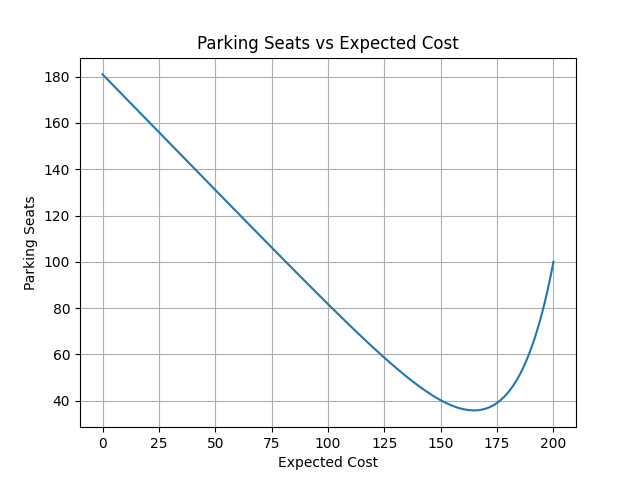
\includegraphics[width=0.8\textwidth]{exercise3.png}
    \caption{Αναπαράσταση του κόστους ανά θέση στάθμευσης}
\end{figure}

\clearpage
\section{Θέμα}

Παρακάτω φαίνεται ο κώδικας \eng{Python} για την επίλυση του προβλήματος
για την εύρεση του βέλτιστου ελεκγτή, για διάφορες τιμές του \eng{discount 
factor} α:

\selectlanguage{english}
\begin{lstlisting}[language=Python]
import numpy as np

def compute_optimal_policy(g, num_states, discount_factor):
    # Initialize the value function array
    V = np.zeros(num_states)
    V_new = np.zeros(num_states)
    # Initialize the policy array
    policy = np.zeros(num_states, dtype=int)
    # Tolerance for convergence
    iters = 0
    while iters < 1000:
        for i in range(num_states):
            # Compute the value for both actions (+1 and -1)
            v_plus = g[i] + discount_factor * (0.5 * V[min(i + 1, num_states - 1)] + 0.5 * V[i])
            v_minus = g[i] + discount_factor * (0.5 * V[max(i - 1, 0)] + 0.5 * V[i])
            # Choose the action with the minimum value
            min_value = min(v_plus, v_minus)
            # Update the policy
            policy[i] = 1 if v_plus < v_minus else -1
            # Update the value function
            V[i] = min_value
            iters += 1
        V = np.copy(V_new)
    return V, policy

if __name__ == '__main__':
    # The given g function
    g = np.array([1, 2, 3, 4, 5, 4, 2, 0, 1, 2])

    num_states = 10

    # different values of a
    base = 0.2
    discount_factors = [base * (i + 1) for i in range(10)]

    for a in discount_factors:
        V, policy = compute_optimal_policy(g, num_states, a)
        print(f'Discount Factor: {a:.1f}')
        print('Optimal Policy:', policy)
        print('Expected Cost:', V)
        print()
\end{lstlisting}
\selectlanguage{greek}

Αντιστοίχως η έξοδος είναι:

\selectlanguage{english}
\begin{verbatim}
Discount Factor: 0.200
Optimal Policy: [-1 -1 -1 -1  1  1  1  1 -1 -1]
Expected Cost: [1.25  2.361 3.596 4.844 6.077 4.693 2.236 0.125 1.125 2.347]

Discount Factor: 0.400
Optimal Policy: [-1 -1 -1 -1  1  1  1  1 -1 -1]
Expected Cost: [1.667 2.917 4.479 6.12  7.661 5.646 2.583 0.333 1.333 2.833]

Discount Factor: 0.600
Optimal Policy: [-1 -1 -1 -1  1  1  1  1 -1 -1]
Expected Cost: [ 2.5    3.929  5.969  8.273 10.176  7.077  3.179  0.75   1.75   3.607]

Discount Factor: 0.800
Optimal Policy: [-1 -1 -1 -1  1  1  1  1 -1 -1]
Expected Cost: [ 5.     6.667  9.444 12.963 14.852  9.778  4.667  2.     3.     5.333]

Discount Factor: 1.000
Optimal Policy: [ 1  1  1  1  1  1  1  1 -1 -1]
Expected Cost: [84.5 83.5 80.5 75.5 68.5 59.5 52.5 49.5 50.5 53.5]

Discount Factor: 1.200
Optimal Policy: [ 1  1  1  1  1  1  1  1 -1 -1]
Expected Cost: [2.07e+08 2.07e+08 2.07e+08 2.07e+08 2.07e+08 2.07e+08 2.07e+08 2.07e+08
 2.07e+08 2.07e+08]

Discount Factor: 1.400
Optimal Policy: [ 1  1  1  1  1  1  1  1 -1 -1]
Expected Cost: [5.125e+14 5.125e+14 5.125e+14 5.125e+14 5.125e+14 5.125e+14 5.125e+14
 5.125e+14 5.125e+14 5.125e+14]

Discount Factor: 1.600
Optimal Policy: [ 1  1 -1 -1 -1 -1 -1 -1 -1 -1]
Expected Cost: [2.152e+20 2.152e+20 2.152e+20 2.152e+20 2.152e+20 2.152e+20 2.152e+20
 2.152e+20 2.152e+20 2.152e+20]

Discount Factor: 1.800
Optimal Policy: [-1 -1 -1 -1 -1 -1 -1 -1 -1 -1]
Expected Cost: [2.104e+25 2.104e+25 2.104e+25 2.104e+25 2.104e+25 2.104e+25 2.104e+25
 2.104e+25 2.104e+25 2.104e+25]
 6.338e+29 6.338e+29 6.338e+29]
\end{verbatim}
\selectlanguage{greek}

Παρατηρείται ότι για τιμές του \eng{discount factor} $a < 1$ η πολιτική
που επιλέγεται είναι πράγματι η ``αναμενόμενη'' ως βέλτιστη. Για τιμές,
μεγαλύτερες του 1, η πολιτική που επιλέγεται δεν είναι απαραίτητα καλή.
Συγκεκριμένα, δυσάρεστο είναι το γεγονός ότι στην κατάσταση 8, η βέλτιστη
επιλογή ανεξαρτήτως κόστους είναι προφανώς να κινηθεί δεξία, δηλαδή στην 9.
Ομοίως στην κατάσταση 6, η βέλτιστη επιλογή είναι να κινηθεί δεξιά, δηλαδή
στην 7. Ωστόσο, το πρόγραμμα δεν βρίσκει αυτές τις απαντήσεις.




\end{document}
